\chapter{The counter example}%%% chapter 3

\textbf{1.}~ In this\pageoriginale chapter we give some counter
examples to the original 14th problem. For this we need some results
on plane curves.  

\setcounter{lem}{0}
\begin{lem}\label{chap3:sec1:lem1}%%% 1
 Let $C$ be a curve of positive genus on the projective plane and let
 $P_1, \ldots , P_m, P_{m+1}, \ldots , P_n \in C(m \geq 1) $ and
 let $P_1, \ldots , P_m $ be independent generic points of $C$ over
 $k(P_{m+1}, \ldots , P_n), $ where $k$ is a field of definition
 for $C$. Then for any set of natural numbers $\alpha_{i} (1 \leq i
 \leq n)$ there does not exist any curve $C'$ such that $C'. C =
 \sum\limits^n_{i=1} \alpha _{i} P_{i}$. 
\end{lem}

\begin{proof}
 Suppose there exists a $C'$ with $C'. C =  \sum\limits_{i=1}^n
 \alpha _{i}. P_{i}$, let $C''$ be a curve of the same degree as
 $C'$ with $C''. C = \sum\limits_{j=1}^l \beta_{j} Q_{j} with Q_{j}$ 
algebraic over $k$. Then $C'. C$ is linearly equivalent to
 $C''. C$ (notation $C' . C \sim  C'' .C)$ on $C$. Hence $
 \sum\limits_{i=1}^m \alpha_{i} P_{i} \sim \sum\limits_{j=1}^l
 \beta_{j} Q_{j} -\sum\limits_{t=m+1}^n \alpha _{t} P_{t}. $ Let $P$
 be any point on $C$. Specializing the above linear equivalence under
 the specialization $(P_1, \ldots , P_m) \rightarrow (P, \ldots ,
 P) $ over $\overline{k} (P_{m+1}, \ldots , P_n)$ (where 
$\overline{k} $ is the algebraic closure of $k$) we get 
$(\sum\limits_{i=1}^m \alpha _{i}) P_\sim \sum\limits_{j=1}^l
 \beta_{j}Q_{j} -\sum\limits_{t=m+1}^n \alpha _{t} P_{t}$. Thus for
 any two points $P,Q$ on $C$, we have $ (\sum \alpha _{i}) P \sim
 (\sum \beta_{i}) Q$. This contradicts the assumption that $C$ has
 positive genus. 
\end{proof}

Here after for a variety $V$, we denote by $K(V)$ the smallest field
of definition for $V$ containing $k$.  

\begin{lem}\label{chap3:sec1:lem2}%%% 2
 Let\pageoriginale $P_1, \ldots, P_t $ be independent generic points
 of the 
 projective plane over a field $k$ and $d$ an integer such that a 
$t < \frac{d^{2}+3d}{2}$. Let $L$ be the linear system of curves
 of degree $d$ passing through $P_{1}, \ldots ,P_{t}$. Let $C$
 be a generic member of $L$ over $k  (P_1, \ldots , P_t)$. Then 
$P_1, \ldots , P_t $ are independent generic points of $C$ over
 $k(C)$. 
\end{lem}

\begin{proof}  
 Set $u = \frac{d^{2}+3d}{2} $. Let $ P_{t+1} ,\ldots , P_{u} $ be
 independent generic points of $C$ over $k(C) \, (P_1, \ldots,
 P_t)$. Then $P_{1}, \ldots , P_{u} $ are independent generic
 points of the projective plane over $k$ as $u$ is the dimension of
 the linear system $L'$ of curves of degree $d$. Let $R_{1}, \ldots ,
 R_{t}$ be independent generic points of $C$ over $k \, (C,
 P_{t+1}, \ldots , P_{u})$. Then we have a specialization 
$(P_{1}, \ldots ,P_{u}) \rightarrow (R_{1} , \ldots , R_{t} ,
 P_{t+1}, \ldots , P_{u}) $ over $k$ because $P_{1} , \ldots ,
 P_{u} $ are independent generic points of the projective plane. Let
 $C$ specialize to $C'$ under this specialization. If $C  \, \neq C'$,
  then $R_1 +\cdots + R_t + P_{t+1}+ \cdots +P_u \subset C.C'$.
 Since $ R_1, \ldots , R_t , P_{t+1}, \ldots , P_u $ are independent
 generic points of $C$ over $k(C)$ and the dimension of the trace 
$L'_{C} $ on $C$ of the linear system $L'$ is $n-1$, we get a
 contradiction. Hence $C = C'$. Thus $(P_{1}, \ldots , P_{t})
 \rightarrow(R_{1}, \ldots , R_{t}) $ is a specialisation over $k(C)$
 and therefore $P_1, \ldots , P_t $ are independent generic points
 of $C$ over $k(C)$. 
\end{proof}

\setcounter{proposition}{0}
\begin{proposition}\label{chap3:sec1:prop1}%%% 1
 Let $P_{1}, \ldots , P_{r} $ be independent generic points of the
 projective plane over the prime field.
\begin{itemize}
\item[{\rm (1)}] Let $C$ be a curve is
 degree $d$ passing through the $P_i $ with multiplicity 
$m_{i}$. Then $\frac{d}{\sum m_{i}} \frac{1}{\sqrt{r}}$, for $r =s^{2}, s \geq 4$. 

\item[{\rm (2)}] Furthermore\pageoriginale if $r'$ is a real number
  such that $r'\, >  \frac{1}{\sqrt{r}}$, then there exists a
  curve $C'$ of degree $d'$ such that $r'  >  \frac{d'}{\sum
    m'_{i}} \; \frac{1}{r}$, where $C'$ passes through $P_{i}$ with with
  multiplicity $m'_{i}$.   
\end{itemize}
\end{proposition}

\begin{proof}
 Let $C$ specialize to $\sigma (C)$ under the specialization $
 (P_1, \ldots , P_r) \rightarrow (P_{\sigma(1)}, \ldots ,
  P_{\sigma(r)})$ where $\sigma$ runs through cyclic
 permutations of $1, \ldots , r$. Considering the curve 
$\underset{\sigma}{\sum} \sigma (C)$, we have only to prove (1) and
 (2) in the case when all the $m_i$ are equal, say $m_i
 =m$. Thus we have to prove that $\frac{d}{m} >  \sqrt{r} =
 s$. If there exists a curve $C$ with $d/m \leq \sqrt{r}$, 
then by suitably raising the degree we can get actually the
equality. Thus (1) is equivalent to:  
\begin{itemize}
\item[{\rm $(1')$}]
 There does not exist a curve of degree sm passing through the 
 $P_i$ with multiplicity at least $m$. 
 
 Similarly (2) is equivalent to: 
 
\item[{\rm $(2')$}] Given $r''\, > \sqrt{r}, $ there exist
  integers $d,  m$ and a curve $C'$ of degree $d$ passing through the
  $ P_i $ with  multiplicity $m$ such that $r'' > \frac{d}{m}
  >  \sqrt{r}$.  
\end{itemize}
\end{proof}

\medskip
\noindent{\textbf{Proof of {\boldmath$(1')$}.}} 
{\textbf{Case (i) s even.}}
 Set $s' =\dfrac{s+2}{2}$. Let $ C_S, C_2, $ and $C'_{S'} $ be
 independent generic curves of degree $s, s' , s'$, respectively.   

\begin{figure}[H]
\centerline{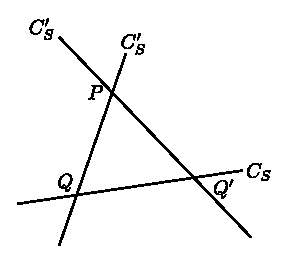
\includegraphics{vol31-figures/fig31-1.eps}}
\end{figure}

Let $C'_{S'} . C_{S'}  = \sum\limits^{s'^2}_{i=1} P_i, C_S . C_{S'} =
\sum\limits^{ss'}_{i=1} Q_i $ 
and $C_{S}. C'_{S} = \sum\limits^{ss'}_{i=1} Q_i$. As the dimension of
the linear system $L^{S'} $ of curves of degree $s'$ is $
\frac{s'^{2}+3s'}{2} > 2s$, among the $P_{i} $ there\pageoriginale
exist $2s$ points say $P_{1}, \ldots , P_{2s} $ which are independent
generic points of the projective plane over $k(C_{s})$. Then by
Lemma \ref{chap3:sec1:lem2} $P_{1}, P_{2}, \ldots , P_{2s}$ are independent generic
points of $ C_{s'}$ over $ k(C_{S}. C'_{S'})$, in fact over $
k(C_{S}, C_{S'}, Q)$ as all the curves considered are independent
generic curves. 
 
 Since $\frac{s^{2}+ 3s}{2} >  2s$, there exist curves of degree
 $s$ passing through the points $P_{1} , \ldots , P_{2s}$. Let $
 C^{*}_{S} $ be the generic curve passing through $P_{1}, \ldots
 ,P_{2s}$. 

\noindent  
\begin{minipage}{4.6cm}
Let 
\begin{align*}
  C_{S'.}C^{*}_{S} & = \sum\limits_{i=1}^{ss'-2s} Q^{*}_{i}+
  \sum\limits_{i=1}^{ss'-2s} P_{i},\\ 
  C'_{S.}C^{*}_{S} & = \sum\limits^{ss'-2s}_{i=1} Q^{*'}_{i}+
  \sum\limits_{i=1}^{2s} P_i. \\ 
\end{align*}
\end{minipage}\hspace{1cm}
\begin{minipage}{3.3cm}
\begin{figure}[H]
\centerline{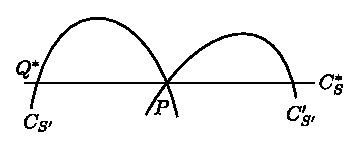
\includegraphics[scale=.8]{vol31-figures/fig31-2.eps}}
\end{figure}
\end{minipage}

By Lemma \ref{chap3:sec1:lem2}, $P_{1}, \ldots , P_{2s}$ are
independent generic points of  
$C^{*}_{S}$. Further, we claim that the $Q^{*}_{i} $ and $Q^{*'}_{i} $
are all distinct. For, consider the linear system $L = 
\big| C^{*}_{S} . C_{S'} - \sum P_{i}\big|$ on $C_{S'}. \sum
Q^{*}_{i} $ is a generic member of $L$. Since degree of $L =
ss' - 2s = 4. \frac{s'^{2} -3s' +2}{2} = 4g(C_{S'}), $ where $
g(C_{S'}) $ denotes the genus of $C_{S'}, L $ has no base
points. Hence each $Q^{*}_{i} $ is a generic points of $C_{s'} $
over $k(C_{s'}, P_{1}, \ldots, P_{2s})$. In particular $Q^{*}_{i}$  do
not lie on $C'_{S'}$. Again 
the degree of the linear system $L -Q^{*}_{i} = ss' - 2s-1 =
4g(C_{S'}) - 1 \geq 2g (C_{S'})$. Hence $L - Q^{*}_{i}$ has no base
point and therefore $Q^{*}_{j} (j \neq i) $ are generic points of $
C_{S'} $ over $k(C_{s'}, Q^{*}_{i})$. Thus $Q^{*}_{i}$ are all
distinct. Similarly considering $C'_{s'}, $ we see 
$Q^{*}_{i},Q^{*'}_{i}$ are all distinct. We may renumber $Q_{i} $
and $Q'_{i} $ such that $Q_{i}, Q'_{i}, 1 \leq i \leq \frac{s' -
 2s}{2}$, are specialized to $Q^{*}_{i}$, $Q^{*'}_{i}$ under the
specialization $(P_{1}, \ldots , P_{2s}, C_{S}) \rightarrow (P_{1},
\ldots , P_{2s}, C^{*}_{S})$ over $k(C_{S},C_{S})$.  

 Assume\pageoriginale that for some $m$ there exists a curve of degree
 $sm$ passing 
 through $r = s^{2} $ independent generic points of the projective
 plane with multiplicity at least $m$. Then there exists a curve $E$
 of degree sm passing through the $P_{i}(1 \leq i \leq 2s)$,  the 
 $Q_{i} (1 \leq i \leq \frac{s^{2}-2s}{2})$ and the $Q'_{i} (1 \leq
 i \leq \frac{s^{2}-2s}{2}) $ with multiplicity at least $m$. Then
 $C_{s'} $ is component of $E$. For otherwise, $E$ $. C_{s'} $ is 
 defined and contains $ \sum\limits^{2s}_{i=1} m P_{i} +
 \sum\limits^{\frac{s^{2}-2s}{2}}_{i = 1} m Q_{i}$. As the degree
 $E. C_{S'}$ is $sms'$, we have $E.C_{s'} =
 \sum\limits^{2s}_{i=1} m P_{i} + \sum\limits^{\frac{s^{2}-2s}{2}}_{i
  = 1} m Q_{i}$. Since the genus of $C_{s'} (= \frac{1}{2} s' (s' -
 3)+1) $ is positive we get a contradiction by Lemma
 \ref{chap3:sec1:lem1}. Hence $C_{s'} 
 $ is a component of $E$. Let $E - C_{s'}$  
 specialize to $E^{*} $ under the specialization $(P_{1}, \ldots ,
 P_{2s}, C_{s}) \rightarrow (P_{1}, \ldots , P_{2s}, C^{*}_{s}).E^{*}$
 is a curve of degree $sm - s'$ passing through  the $ P_{i} (1 \leq i 
 \leq 2s) $ and the $Q^{*}_{i}(1 \leq i \leq \frac{s^{2}-2s}{2}) $
 with the the multiplicity at least $(m-1)$ and through $Q'^{*}_{i}
 $ with the multiplicity at least $m$. We shall show the non-existence
 of such a curve by induction on $m$. We assert that $C^{*}_{s} $ is
 component of $E^{*}$. For, if not, $E^{*}. C^{*}_{s} $ is defined
 and contains 
 $$ 
 \sum\limits^{2s}_{i=1} (m -1) P_{i} + 
 \sum\limits^{\frac{s^2-2s}{2}}_{i=1} (m-1) Q^{*}_{i} +
 \sum\limits^{\frac{s^2 - 2s}{2}}_{i=1} m  Q^{*'}_{i}.
 $$ 
Inspecting the degrees we see that 
$$ 
E^{*} . C_{s} =
 \sum\limits^{2s}_{i=1} (m-1)P_{i}+
 \sum\limits^{\frac{s^{2}-2s}{2}}_{i=1} (m-1) Q'_{i} +
 \sum\limits^{\frac{s^{2}-2s}{2}}_{i=1} m Q^{*'}_{i}.
$$ 
  Hence $((m -1) C_{s'} + m C'_{s'} - E^{*}) . C^{*}_{s} =
 \sum\limits^{2s}_{i=1} m P_{i}$. As the genus of $C^{*}_{S}(=
 \frac{1}{2} s (s-3)+1)$ is positive and since the $P_{i}$ are
 independent generic points of $C^{*}_{s}$ by lemma
 \ref{chap3:sec1:lem2}, we have a  contradiction by Lemma \ref{chap3:sec1:lem1}.  
 
 Hence\pageoriginale $C^{*}_{s}$ is a component of $E^{*}$. If $m =
 1$, degree of $E^{*}$ is  $s-s'$. 

Hence we get a contradiction. If $m \, > 1$, then $E^{*}-
C^{*}_{S.}$ is of degree $s(m-1) -s'$ and passes through the $P_{i},
Q^{*}_{i}$, with multiplicity at least $m-2$, $m-2$ and $(m-1)$
respectively. Hence by induction hypothesis $E^{*}- C^{*}_{S.}$ does
not exist and the lemma is proved, when $r$ is even 


\medskip
\noindent \textbf{Case (ii) $s$ odd.}
 Set $s' = \frac{s+1}{2}$. Let $C_{S}, C_{S'} C'_{S'}$ be independent
 generic curves. Let $P_{1}, \ldots ,P_{s}$ be $s$ points contained
 in $C_{S'}. C'_{S'}$. We take a generic curve $C^{*}_{S}$ of
 degree $s$ passing through $P_{1}, \ldots ,P_{s}$ and proceed as
 in (i). We omit the details. 


\begin{remark*}
 We remark that Proposition \ref{chap3:sec1:prop1} is not true for $ r
 \leq 9$. The 
 following are the example to that effect. (1) For $r = 1,2$, a line
 passing through the $P_{i}$ (2) $r = 3$, a line passing through
 two of the $P_{i}$ (3) $r= 4, 5$, a conic through the $ P_{i} $
 (4) $r =6$, a conic through 5 of the $ P_{i}$ (5) $r = 7$, a cubic
 having a double point at one of the $ P_{i} $ and passing through
 all the $ P_{i}$. (6) $r = 8$, a curve of degree 6 having a triple
 point at one of the $ P_{i} $ and double points at all the $P_{i}$
 (7) $r = 9$, a cubic passing through all the $P_{i}$. 
\end{remark*} 

Furthermore it is not known if $r \geq 9$, is sufficient to ensure
the inequality of Proposition \ref{chap3:sec1:prop1}. 


\medskip
\noindent \textbf{Proof of {\boldmath$(2')$.}}
 Let $L^{d} $ be the linear system of curves of degree $d$. Let $
 f(x_{0}, x_{1},x_{2})$ be a homogeneous polynomial of degree $d$. The
 condition that the curve defined by $f$ should pass through a point
 $p$ with multiplicity $m$ imposes $\frac{m(m+1)}{2}$ linear
 conditions (not necessarily independent). 

Thus\pageoriginale 
$$
\displaylines{\hfill 
\dim ( L^{d} - \sum\limits^{r}_{i=1} m P_{i}) \geq \frac{d(d+3)}{2} - r
\frac{m(m+1)}{2} \geq 0\hfill \cr 
\text{if}\hfill 
\frac{d(d+3)}{2} \geq r \frac{m(m+1)}{2}.\hfill }
$$ 
i.e. if $m \geq \dfrac{r-3(\frac{d}{m})}{(\frac{d}{m})^{2}-r}$. Now
choose a rational number $\lambda $ such that $r'' >  \lambda
> \sqrt{r}$. Writing $ \lambda = \frac{d}{m} $ with sufficiently
large m we get a curve $C'$ of degree d passing through the $P_i$
with multiplicity $m$ such that $r'' >  d/m > \sqrt{r}$
and ($2'$) is proved. 

\medskip
\noindent{\textbf{2.}}
 We now proceed to give the counter example where the transcendence
 degree of the sub-field $L_G $ of invariants is four.  

Let $a_{ij}, i = 1,2,3, j = 1, \ldots , r$ be algebraically
independent elements over the prime field $\Pi$ . Let $k$ be a field
containing the $a_{ij}$. Consider the projective plans $S$ over
$k$. Set $P_{i} = (a_{1i}, a_{2i}, a_{3i}), P_{i} \in S, i =
1,2,\ldots ,r$. Then the $P_{i}$ are independent generic points of
$S$ over the prime field . Let $ x_{1}, \ldots , x_{r}, y_{1}, \ldots
,y_{r}$ be algebraically independent elements over $k$. Consider the
subgroup $G$ of $GL (2r, k)$ given by 
\begin{multline*}
 G = \left\{ \sigma \in GL (2r, k) \bigg| \sigma = 
 \begin{pmatrix}
 B_1 & & 0 \\ 
& \ddots & \\
 0 & &  B_r 
\end{pmatrix},\right. \\ 
 \left.B_i = \begin{pmatrix}
 c_i & c_i b_i\\
0 & c_i 
\end{pmatrix},
 \sum\limits^{r}_{i=1} b_{i} a_{ji} = 0, \; j =1, 2,
 3, \; \prod\limits^{r}_{i=1} c_{i} = 1\right\}. 
\end{multline*}

The group $G$ acts on $k[x_{1}, y_{1},\ldots , x_{r}, y_{r}]$ with $
\sigma (x_{i}) = c_{i}(x_{i}+b_{i}y_{i})$, $\sigma(y_{i}) = c_{i} y_{i},
i =1, \ldots , r$.  
  
\setcounter{thm}{0}
\begin{thm}\label{chap3:sec2:thm1}%%% 1
 The\pageoriginale ring of invariants $I_G$ is not finitely generated
 the $k$. Set $ t= y_1 , \dots , y_{r}, u_{ i} = t/y_i$, $v_i = x_i u_i$
 and $w_j = \underset{i=1}{\overset{r}{\sum}} a_{ji}v_i$. We need
 some lemmas.  
\end{thm}


\setcounter{lem}{0}
\begin{lem}\label{chap3:sec2:lem1}%%% 1
 $I_G = k [x_1, y_1, \dots , x_r, y_r]\cap k(w_1, w_2, w_3, t)$.
\end{lem}

\begin{proof}
 It is sufficient to prove that the invariant sub-field 
 $L_G = k(w_1, w_2, w_3, t) $. A straight forward verification
 shows that $ w_1, w_2, w_3, t \in L_G$. Hence $ k(w_1, w_2, w_3,
 t) \subseteq L_G$ as $ a_{ij}$ are independent over $ \prod$, we
 have $ k(x_1, \dots , x_r, y_1, \dots , y_r) = k(w_1, w_2, w_3,
 x_4, \dots , x_r, y_1 , \dots , y_r)$. Now $G$ operates on $k[
  w_1, w_2, w_3, x_4, \dots , x_r, y_1, \dots , y_r ]$. As $w_i,
  t \in L_G$, to compute $L_G$ it is enough to consider the action of $G$
 on $k(w_1, w_2, w_3, t)$  $[ x_4, \dots , x_r, y_1, \dots , y_{r-1}
 ]$. Consider the subgroup $H$ of $G$ consisting of elements $\sigma$ of
 G for which $c_i = 1, i=1, \dots , r, b_i = 0, i \ge 5$ and
 $b_4$ arbitrary. Since $H$ is infinite, $k(w_1, w_2, w_3, t, x_4,
 \dots , x_r, y_1, \dots , y_{r-1})$ is a transcendental extensions
 of $ L_H$ the fixed field of $H$. Now, $L_H \supseteq k(w_1,
 w_2, w_3, t, x_5, \dots , x_r, y_1, \dots , y_{r-1})$. Therefore
 $ L_H = k(w_1, w_2, w_3$, $t, x_5, \dots , x_r, y_1, \dots ,
 y_{r-1})$. Next we consider the action of $G$ on $k(w_1, w_2, w_3,
 t) [ x_5, \dots , x_r,y_1, \dots , y_{r-1} ]$ and consider the
 subgroup $H_1$ of $G$ consisting of elements $\sigma$ of $G$ with $
 b_i = 0, i \ge 6, c_i = 1, i = 1, \dots , r$. The fixed field $
 L_{H_1}$ of $H_1 $ is $ k(w_1, w_2, w_3, t, x_6, \dots , x_r,
 y_1, \dots , y_{r-1})$. Proceeding in the same way we arrive at
 $k(w_1, w_2, w_3, t, y_1, \dots , y_{r-1})$. Consider $ k(w_1, 
 w_2, w_3, t) [ y_1, \dots , y_{r-1} ]$. $\sigma \in G$ acts on $
 k(w_1, w_2, w_3,t)$ $[y_1, \dots , y_{r-1}]$ with $ \sigma (y_i) =
 c_i y_i , i=1, \dots , r-1$, where $ c_i$ are arbitrary non-zero
 elements of $k$. Hence $ L_G = k(w_1, w_2, w_3,t)$. 
\end{proof}

As $ w_1, w_2, w_3 $ are algebraically independent over $k$, we may
regard $ H = k [w_1, w_2, w_3]$ as the homogeneous coordinate ring of
the projective\pageoriginale plans $S$. Let $\mathscr{F}_i = (z_i,
z'_i)$ denote the prime ideal is $H$ corresponding to the point $
P_i$, where $ z_i = 
a_{3i} w_1 - a_{1i} w_3, z_{i}^{\prime} = a_{3i} w_2 - a_{2i}
w_3$. Set $\mathcal{W}_n = \underset{i=1}{\overset{r}{\cap}}
\mathscr{Y}_{i}^{(n)} $, for $n > 0$ and $ \mathcal{W}_n = H $, for
$n\le 0$. 

\begin{lem}\label{chap3:sec2:lem2}%%% 2
 $ I_G = \bigg\{\underset{n}{\sum}a_n t^{-n} \mid a_n \in \sqcap_n
  \bigg\}$.

Assuming Lemma \ref{chap3:sec2:lem2} we shall first prove Theorem
\ref{chap3:sec2:thm1} 
and later prove Lemma \ref{chap3:sec2:lem2}. Suppose $ I_G$ is
finitely generated, say $ I_G = k[f_1, 
 \dots , f_m]$. We may assume $ f_j = h_j t^{-j} , h_j \in \mathcal
{W}_j , h_j$ homogeneous, $ j=1, \dots , m$. Set $ r_j =
\dfrac{\text{degree } h_j}{j}$, $j = 1, \dots , m$ and $ r^* = \underset{i\le
  j\le m}{\min} 
r_j$. For any monomial $ f_{1}^{i_1} \dots f_{m}^{i_m}=
h_{1}^{i_1}\dots h_{m}^{i_m} t^{-i_1 - 2i_2 - \dots - mi_m}$, we have
$ \dfrac{\text{degree } (h_{1}^{i_1}\dots h_{m}^{i_m})}{i_1 + 2i_2 +
 \cdots + mi_m} \ge r^*$. Hence for any homogeneous $ a_n \in
\mathcal{W}_h$, we have $ \dfrac{\text{degree } a_n}{n} \ge r^*$. By
proposition \ref{chap3:sec1:prop1}, $r^* > s = \sqrt{r}$, for $ r \ge 4$. Again by
the same proposition there exists an $a_n \in \mathcal{W}_n$, for some $n$,
such that degree $ a_{n/n} <  r^*$. This is a contradiction and
therefore $ I_G$ is not finitely generated. 
\end{lem}

It now remains to prove Lemma \ref{chap3:sec2:lem2}. We first prove
\begin{equation*}
I_G \subseteq \bigg\{ \underset{n}{\sum} a_n t^{-n} \mid
a_n  \in H \bigg\}. \tag*{($\ast$)} 
\end{equation*}
As $ a_{ij}$ are algebraically independent over $k$ we have 
$$
k [v_1, \dots , v_r] = k[w_1, w_2, w_3, v_4, \dots , v_r].
$$ 

Hence 
\begin{multline*}
 k \left[x_1, \dots, x_r , y_1 . . y_r , \dfrac{1}{y_1}, \dots ,
  \frac{1}{y_r}\right]\\ 
 = k \left[ w_1, w_2, w_3, x_4, \dots , x_r, y_1,
  \dots y_r, \frac{1}{y_1}, \dots , \frac{1}{y_r} \right].
\end{multline*}

Now 
\begin{multline*}
 k \left[ w_1, w_2, w_3, x_4, \dots , x_r, y_1, \dots y_r ,
  \frac{1}{y_1}, \dots , \frac{1}{y_r} \right]\\ 
 \bigcap k(w_1, w_2, w_3, y_1, \dots , y_r) 
 = k \left[ w_1, w_2, w_3, y_1, \dots , y_r,
  \frac{1}{y_1}, \dots , \frac{1}{y_r} \right].
\end{multline*}

 Now by lemma \ref{chap3:sec2:lem1}, 
\begin{align*} 
 I_G & \subseteq k \left[ w_1, w_2, w_3, y_1, \dots , y_r,
  \frac{1}{y_1}, \dots , \frac{1}{y_r} \right] 
 \bigcap k(w_1, w_2, w_3, t)\\  
 & = k \left[ w_1, w_2, w_3, t, \frac{1}{t}, y_2 , \dots , y_r, \frac{1}{y}_2
 , \dots , \frac{1}{y_r} \right] \bigcap k(w_1, w_2, w_3,t)\\ 
 & = k \left[ w_1,
 w_2, w_3, t, \frac{1}{t} \right]. 
\end{align*}\pageoriginale

Hence \quad $I_G  \subseteq \left\{ \sum\limits_n a_n t^{-n} \big| a_n
\in H \right\}$. Let $\mho_i$ be the valuation ring $k [y_1, \dots ,
  x_r,  y_1, \dots , y_r]_{(y_i)}, 1\le i \le r$ and let $V_i$ be the
corresponding normalized valuation. We prove
\begin{equation*}
 \mathscr{Y}_{i}^{m}= \mathscr{Y}_{i}^{(m)}= \bigg\{ f \in H \mid V_i
(f) \ge m \bigg\}, \tag*{$\ast\ast$}
\end{equation*}
for every $m$. Since $ z_i = \underset{j \ne i}
{\sum} (a_{3i} a_{1j} - a_{1i} a_{3j}) x_j u_j, V_i
(z_i)=1$. Similarly $V_i (z_{i}^{\prime})= 1$. It is easy to
check that $ w_3, z_i /t$, and $ z_{i}^{\prime}/t$ modulo the
maximal ideal $\mathscr{M}_i$ of $\mho_i$ are algebraically
independent over $k$. Now $k[w_1, w_2, w_3] = k [z_i,
 z_{i}^{\prime}, w_3]$. If $ h \notin \mathscr{Y}_i$, then $
h \equiv h_1 \pmod {\mathscr{M}_i}$, with $ 0\ne h_1 \in k [w_3]$. Hence $
V_i(h)=0$. Therefore $\mathscr{Y}_{i}^{(m)} \subseteq \bigg\{ h
\in H \mid V_i (h) \ge m \bigg\}$. To prove $(\ast\ast)$ we
need only to prove that, for $f \in H$, $V_i (f) \ge m$ implies
$ f \in \mathscr{Y}_{i}^{m}$. This in turn will be proved if we
prove that $f \in \mathscr{Y}_{i}^{m}$, $f \notin
\mathscr{Y}_{i}^{m+1}$ implies $ V_i (f)=m$. 
 If $ f\in \mathscr{Y}_{i}^{m}$, $f\notin \mathscr{Y}_{i}^{m-1}$ then $f$ can be
 written as $f = \sum\limits^m_{j=}h_j z_{i}^{j}
 z_{i}^{\prime^{m-j}}$, with $ h_j \in k[w_3]$, $h_l \ne 0 \mod
 \mathscr{M}$, for  some $l$. Hence $ f/z_{i}^{\prime m} = \sum\limits^m_{j=0} h_j
 (\frac{z_i}{z_i})^j$. As $z_i/z_{i}^{\prime}$ and $w_3$ modulo
 $m_i$ are algebraically independent over $k, f/z_{i}^{\prime^{m}}
 \not\equiv 0 \pmod {\mathscr{M}_i}$. Hence $V_i (f)=
 V(z_{i}^{\prime^{m}})=m$ and 
 $(\ast\ast)$ is proved. Next, we prove 
\begin{equation*}
V_i (\underset{n}{\sum}a_n t^{-n})= \underset{n}{\min} V_i (a_r
t^{-n}),
\end{equation*}
 for $a_n \in H$. Let $ d = \underset{n}{\min}$ $V_i (a_n t^{-r})
 $. For every\pageoriginale $n$, $V_i (a_n t^{-n})\ge d$ i.e. $V_i
 (a_n)\ge n+d$. Hence by $(\ast , \ast)$, $a_n \in
 \mathscr{Y}_{i}^{n+d}$. Let $a_n = \sum\limits^{n+d}_{j=0} h_{nj}
 z_{i}^{j} z_{i}^{\prime n+d-j}$. Then $\sum\limits_n
 \frac{a_n}{t^{n+d}} = \sum\limits_n 
 \sum\limits_j h_{nj} (\frac{z_i}{t})^j (\frac{z_{i}^{\prime}}
{t})^{n+d-j} $. If $V_i (a_m t^{-m}) = d$ for some $m$,
then $ 0 \ne h_{ml} \mod \mathscr{M}_i \in k[w_3] $ for
some $l$. Since $ z_i/t$ and $ z_{i}^{\prime}/t$ 
modulo $\mathscr{M}_i $ are algebraically independent
over $ k (w_3 \mod \mathscr{M}_i)$, $\sum\limits^m_n
\frac{a_n}{t^{n+d}} \not\equiv 0 \pmod {\mathscr{M}_i}$. Hence $V_i
(\sum\limits_n a_n t^{-n})=d $.  

 Now suppose $f \in I_G$. Then by $(\ast) f$ can be written as $f =
 \sum\limits_n a_n t^{-n}$, $a_n \in H$. As $I_G \subseteq \mho_i , 1 
 \le i \le r, V_i (f)\ge 0$. Hence by $ (\ast \ast \ast )$, $V_i (a_n
 t^{-n}) \ge 0$, that is $V_i (a_n)\ge n$ and $a_n \in
 \mathscr{Y}_{i}^{n}$. Hence $I_G \subseteq \bigg\{ \sum a_n
 t^{-n}\mid a_n \in \mho_n \bigg\}$. On the other hand if $ a_n \in
 \mathscr{W}_n$, then $V_i (a_n) \ge n, i =1, \dots , r$. Hence $a_n$
 is divisible by $t^n$. Thus $ I_G \supseteq \bigg\{ \sum 
 a_n t^{-n} \mid a_n \in \mathscr{W}_n \bigg\} $ and the proof of
 Lemma \ref{chap3:sec2:lem2} is complete.


\medskip
\noindent\textbf{3.} \quad  In the counter example we have given to
the original $14^{\text{th}}$ problem in section 2, the group $G$ is
commutative. In this section we give an example, where the group $G$
is such that $[G, G] = G$.  

If we make use of the structure of the ring $I_H$ of invariants of
the subgroup $H$ of $G$ given in the last section such that all the 
$c_i$ are 1 then we can give a direct construction of the required
example. But since we did not give the explicit structure of $I_H$,
we do it in an indirect way. 

Let $ a_{ij}$, $i = 1, 2, 3$, $j = 1, \dots , r (r = 16)$ be
algebraically independent real numbers over the field of relational
numbers. Set 
 
$V= \Bigg\{ (b_1 , \dots , b_r) \mid b_i ~ \text{real,} ~ 
\sum\limits_j a_{ij} b_{j} = 0 (i = 1, 2, 3, s =$\pageoriginale an
even number $\ge 4$, 
$$   
G_o = \left \{ 
\begin{pmatrix}   
 c_1 B_1 & & \bigcirc\\ 
 & \ddots & \\ 
 \bigcirc & & c_r B_r
\end{pmatrix} 
B_i = 
\begin{pmatrix}   
 1 & \dots\dots & b_{il}\\ 
 \ddots & 0 & \\ 
 & \ddots & b_{is} \\ 
 0 & & 1 
\end{pmatrix},~ 
\begin{matrix}
 (b_{li}, \dots , b_{ri}) \in V,\\ 
 c_i ~\text{ real}, \prod_{c_i} = 1
\end{matrix} \right \}
$$ 

Let $K$ be the real number field. $G_o$ acts on the polynomial
ring
{\fontsize{10pt}{12pt}\selectfont
$$
R_0 = K [ x_{11},x_{12}, \dots , x_{1s}, y_1, x_{21}, x_{22}, \dots ,
 x_{2s}, y_2 , \dots , x_{r1}, x_{s2}, \dots , x_{rs}, y_r ].
$$}\relax
Let $I_0$ be the ring of $G_o$ - invariants in $R_o$. Then setting $
t = \prod y_j$ 
 \begin{enumerate}[(i)]
 \item $w_{ij} = \underset{\alpha} {\sum} a_{i \alpha} x_{\alpha j}
  t/y_{\alpha}\in I_o$ 

 \item $I_o = R_o \bigcap K(w_{11}, \dots, w_{1s}, \;\; w_{21}, \dots,
   w_{2s}, \;\; w_{31}, \dots , w_{3s}, t)$.  
 \end{enumerate}

 Since $I_o / I_o \bigcap (\underset{j\ge 2}{\sum} x_{ij}R)$ is
 isomorphic to previous example $I_G$, we see that $I_o$ is not
 finitely generated. We see also easily that every element of $I_o$
 can be expressed in the form $\sum\limits_i a_i t^{-i}$ (finite sum)
 such that $a_i \in \mathscr{Y}= K [w_{11}, \dots , w_{3s}]$, $a_i
 t^{-i} \in I_o$. 
 
 For each $T \in SL (s, K)$, let 
\begin{align*}
  T_r & = 
  \begin{pmatrix} 
    T^{\prime} & & 0\\ & \ddots & \\  0 & & T^{\prime} 
  \end{pmatrix} , T^{\prime} = 
  \begin{pmatrix} 
   T & 0\\ \\ 0 & 1 
  \end{pmatrix}\\ 
  & \hspace{2cm}(T^{\prime} \in SL (s+1, K)), T_r \in SL(r(s+1),K)\\
  \text{and}\quad  G_1 & = \bigg\{ T_r \mid T \in
 SO (s, K) \bigg\}. 
\end{align*}

Then one can easily see that $ I_o$ is
 $G$-admissible and the module $ M_i = \sum\limits_{j} w_{ij} K$ is also $
 G_1$-admissible and $T$ is the transformation on $N_i$ given by
 $T_r$. Therefore for a general linear transformation $T \in SL (s,
 K)$ we have $I_{o/I_o \cap (\sum\limits_{j \ge 2} x_{ij}R)} T$ is
 isomorphic to the previous example $ I_G$. 
 
 Therefore we see that the degree $a_i > 4i$ (for $i >
 0$) and that for any rational number $\alpha$ greater than
 $\frac{1}{4}$. there is a homogeneous form $a_l$ in 
$w_{ij}$\pageoriginale such that $\frac{\deg ~ a_l}{r_l}= \alpha$ and
 $a_l t^{-l}\in I_o$.  
 
 Now consider a copy of $R_o$ say $R'_{o}$. The isomorphism
 of $R_o$ onto $R_{o}^{\prime}$, we denote by ``/''. Let $ G_2$ be
 the subgroup in $SL (2r(s+1),K)$ generated by 
\begin{align*}
  G_{o}^{\ast} & = \left\{ \begin{pmatrix}  B_{1} & 0 \\  0 &
    B_{2} \end{pmatrix} \mid B_i \in G_o \right\}  ~(\text{i.e.}~
  G_{o}^{\ast} = G_o \times G_o)\\ 
  G_{1}^{\ast} & = \left\{ \begin{pmatrix} T & 0 \\ 0 & T \end{pmatrix}
  \mid T \in G_1 \right\}. 
\end{align*}
Then the ring of $G_{o}^{\ast}$- invariants
 is $ I_o \otimes I_{o}^{\prime}$. Let $M_{id}$ be the module of
 homogeneous forms $ a_i$ in $\mathscr{Y}$ of degree $d$ such that $ a_i
 t^{-1}$ is in $ I_o$. Then each $ M_{id}$ which is not zero defines a
 representation of $G_1$. Hence we can choose a linearly independent
 basis of $M_{id}$ say $f_{idl} , \ldots , f_{idn} (i,d)$ such that
 the representation is orthogonal. Then $ f_{id}^{\ast}= \sum\limits_j
 f_{idj}f_{idj}^{\prime}$ is $G_{1}^{\ast}$-invariant and $
 f_{id}^{\ast}t^{-i}$ is $ G_2$-invariant. Therefore the same
 reasoning as in the previous example $I_G$ can be applied to the
 ring $ I_2$ of $G_2$-invariant and we see that $I_2$ is not
 finitely generated. 
 
 Let $C$ be the complex number field and let $\bar{G_2}$ be the
 closure of $ G_2$ in $SL(2r(s+1),C)$. We want to show that
 $\bar{G_2}$ contains a connected normal algebraic subgroup $
 \bar{G}$ such that 
 \begin{enumerate}[(i)]
 \item $ \bar{G_2}/ \bar{G}$ is a torus group and 

 \item $[\bar{G}, \bar{G}] = \bar{G}$
\end{enumerate}
 
 If the existence of $\bar{G}$ is shown then $\bar{G}$
 is the given example. 
 
 Let ${G}_{oo}$ be the subgroup of $G_0$ defined by $c_1 = \ldots =
 c_r = 1$. Then we can consider the same construction as done for
 $G^*_0,G_2$  and $\bar{G}_{20}$.   
 
 We claim that $\bar{G}_{20}$ is the required $\bar{G}$.

 \begin{proof}
   Since\pageoriginale $\bar{G}_{20}$ is normal in $G_2$ we see
   that  $\bar{G}_{20}$ is normal in  
   $\bar{G}_{2}$. Obviously $\bar{G}_{2} /
   _{\bar{G}_{20}}$ is a torus group. It is also obvious that
   $\bar{G}_{20}$ in connected. Therefore we have only to show
   that $[\bar{G}_{20},\bar{G}_{20}]\supseteq
   \bar{G}_{20}$. Since
   $[\bar{G}_{20},\bar{G}_{20}]$ is a closed subgroup we
   have only to show that both $G^*_1$  and $G^*_{oo}$ are in
   $[\bar{G}_{20},\bar{G}_{20}]$. Since $G^*_1$ is
   semi-simple and since $G^*_1 \subseteq \bar{G}_{20}$ we see that $G^*_1
   \subseteq [\bar{G}_{20},\bar{G}_{20}]$. Consider the
   set $\{B^*_1\}= \bigg\{\begin{pmatrix} B & O\\ O& E \end{pmatrix}
   \bigg \}$ ($E$ =identity in $SL (x(s+1),k) B \in G_{\infty}$). For a
   fixed $T^* \in G^*_1, B^*_1 \rightsquigarrow T^{*-1} B^{*-1}_1
   T^* B^*_1$ gives a homomorphism $B^*_1$ and $B^*_1$ (because
   $B^*_1$ is isomorphic to a vector space over $K$). Since s is even,
   there is a $T^* \in G^*_1$ such that $T^{*-1} B^{*-{1}}_1 T^*
   B^*_1= \begin{pmatrix} E& O\\ O& E \end{pmatrix}$ implies
   $B^*_1= \begin{pmatrix} E& O\\ O& E \end{pmatrix}$. Therefore we
   see that image is dense in $B^*_1$. Therefore
   $[\bar{G}_{20},\bar{G}_{20}]$ contains the set
   $\{B^*_1\}$. Similarly $[\bar{G}_{20},\bar{G}_{20}]$
   contains all the $\begin{pmatrix} E& O\\ O& B \end{pmatrix},(B \in
   G_{oo})$. Therefore $[\bar{G}_{20},\bar{G}_{20}]$
   contain $G^*_{oo}$ and the proof is complete. 
 \end{proof}
